% !TeX program = lualatex
% このファイルは LuaLaTeX で処理してください(pdfLaTeX/upLaTeXでは動作しません)。
\documentclass[a4paper,11pt]{ltjsarticle}

\usepackage{amsmath,amssymb,mathtools}
\usepackage{ascmac}
\usepackage{siunitx}
\usepackage{geometry}
\geometry{a4paper,top=15mm,bottom=18mm,left=14mm,right=14mm}
\usepackage{tikz}
\usetikzlibrary{arrows.meta,positioning,calc,decorations.pathreplacing}
\usepackage[most]{tcolorbox}
\usepackage{booktabs}
\usepackage{array}
\usepackage{enumitem}
\usepackage{pdfpages}
\usepackage{fontspec}
\newfontfamily\musicfont{Segoe UI Symbol}

\setlength{\parindent}{0pt}
\setlength{\parskip}{2pt}
\renewcommand{\arraystretch}{1.25}

\newtcolorbox{defbox}[1][]{%
  colback=black!3,colframe=black,boxrule=0.6pt,arc=1mm,
  left=6pt,right=6pt,top=4pt,bottom=4pt,#1}

\newcommand{\banner}[1]{%
  \begin{tcolorbox}[colback=black,coltext=white,boxrule=0pt,sharp corners,
    left=8pt,right=8pt,top=5pt,bottom=5pt,before skip=8pt,after skip=8pt]
    {\Large\bfseries #1}
  \end{tcolorbox}}

\newcommand{\subbanner}[1]{%
  \begin{tcolorbox}[colback=black!80,coltext=white,boxrule=0pt,sharp corners,
    left=8pt,right=8pt,top=4pt,bottom=4pt,before skip=6pt,after skip=6pt]
    {\large\bfseries #1}
  \end{tcolorbox}}

\newtcolorbox{pointbox}[1][]{%
  colback=black!4,colframe=black,boxrule=0.6pt,arc=1mm,
  left=6pt,right=6pt,top=4pt,bottom=4pt,#1}

\pagestyle{plain}

\begin{document}

\banner{リコーダーの音階と固有振動数}

　管にはその長さと形状に応じた固有振動数があり，管楽器に分類される楽器はその性質を利用して狙った音階の音を奏でる。リコーダーも固有振動の性質を応用した楽器の1つであり，
その形状は下端と，吹き口近くにある窓がともに開口となる開管と見なすことができる。\\
　乾燥した室温17.5℃の部屋において，図(a)のようにリコーダーの指穴をすべて閉じると，吹いて出る音（基本振動）の振動数は $3.5\times10^{2}\,\mathrm{Hz}$ であった。
\textgt{登場する数値を目の前の現実の世界と結び付けてイメージしながら各設問に答えよ。}このとき，気温 $t$[℃]の下での空気中の音速は $V=331.5+0.6t\,[\mathrm{m/s}]$ と近似できることを利用してよい。開口端補正は考えないものとする。\\
　特に指定がない限り求める物理量は有効数字2桁で計算せよ。計算には，電卓を用いてもよい。


\begin{center}
\begin{tikzpicture}[x=0.9cm,y=0.55cm]
  % ---- (a) 指穴をすべて閉じた状態 ----
  \begin{scope}
    % 管本体の輪郭（マウスピースの嘴形を丸みのある曲線で表現し，胴体は緩やかなテーパー，
    % 足部管は丸みを帯びたベル状に裾広がりする，実物に近いシルエット）
    \draw[thick]
      (-0.32,9.5)
      -- (-0.32,9.68)
      -- (-0.14,9.88)
      -- (0.14,9.88)
      -- (0.32,9.68)
      -- (0.32,9.5)
      -- (0.4,8.95)
      -- (0.4,8.6)
      -- (0.5,1.3)
      to[out=-90,in=110] (0.72,0.35)
      to[out=-70,in=90]  (0.72,0)
      -- (-0.72,0)
      to[out=90,in=-110] (-0.72,0.35)
      to[out=70,in=-90]  (-0.5,1.3)
      -- (-0.4,8.6)
      -- (-0.4,8.95)
      -- cycle;
    % 頭部管・中部管の継ぎ目（二重リング）
    \draw[thin] (-0.4,8.9) -- (0.4,8.9);
    \draw[thin] (-0.4,8.78) -- (0.4,8.78);
    % 中部管・足部管の継ぎ目
    \draw[thin] (-0.5,1.3) -- (0.5,1.3);
    % 窓（ラビウム。塗りつぶさず輪郭のみ）
    \draw[thick]
      (-0.14,8.6) -- (0.14,8.6) -- (0.14,8.4)
      to[out=-90,in=0] (0,8.22)
      to[out=180,in=-90] (-0.14,8.4) -- cycle;
    % 指穴（下から1〜7番目。すべて閉じているので黒丸＝塞いだ状態）
    \foreach \y in {1.8,2.6,3.4,4.2,5.0,5.8,6.6} {
      \fill (0,\y) circle (0.09);
    }
    % 左手・右手の範囲を示す波括弧
    \draw[decorate,decoration={brace,amplitude=5pt,mirror}] (0.85,4.6) -- (0.85,7.0);
    \node[right,font=\small] at (1.05,5.8) {左手};
    \draw[decorate,decoration={brace,amplitude=5pt,mirror}] (0.85,1.4) -- (0.85,3.8);
    \node[right,font=\small] at (1.05,2.6) {右手};
    % 窓のラベル（右横から短い引き出し線でつなぐ）
    \draw[thin] (0.14,8.5) -- (1.3,8.5);
    \node[right,font=\small] at (1.3,8.5) {窓（開口端）};
    % 下端のラベル
    \node[below,font=\small] at (0,-0.2) {開口端};
    % 長さLの両矢印（窓の中央〜下端）：他の要素と重ならないよう左側にさらに離して配置
    \draw[<->,>=stealth] (-1.8,8.5) -- (-1.8,0);
    \node[left,font=\small] at (-1.8,4.2) {$L$[m]};
    \node[below,font=\large] at (0,-1.1) {(a)};
  \end{scope}

  % ---- (b) 右手の指穴をすべて開いた状態（開口端が下から4番目の指穴まで上がる） ----
  \begin{scope}[xshift=5.4cm]
    \draw[thick]
      (-0.32,9.5)
      -- (-0.32,9.68)
      -- (-0.14,9.88)
      -- (0.14,9.88)
      -- (0.32,9.68)
      -- (0.32,9.5)
      -- (0.4,8.95)
      -- (0.4,8.6)
      -- (0.5,1.3)
      to[out=-90,in=110] (0.72,0.35)
      to[out=-70,in=90]  (0.72,0)
      -- (-0.72,0)
      to[out=90,in=-110] (-0.72,0.35)
      to[out=70,in=-90]  (-0.5,1.3)
      -- (-0.4,8.6)
      -- (-0.4,8.95)
      -- cycle;
    % 頭部管・中部管の継ぎ目（二重リング）
    \draw[thin] (-0.4,8.9) -- (0.4,8.9);
    \draw[thin] (-0.4,8.78) -- (0.4,8.78);
    % 中部管・足部管の継ぎ目
    \draw[thin] (-0.5,1.3) -- (0.5,1.3);
    % 窓（ラビウム。塗りつぶさず輪郭のみ）
    \draw[thick]
      (-0.14,8.6) -- (0.14,8.6) -- (0.14,8.4)
      to[out=-90,in=0] (0,8.22)
      to[out=180,in=-90] (-0.14,8.4) -- cycle;
    % 右手側（下から1〜4番目）は開いたので白丸＝開いた状態，左手側（5〜7番目）は閉じたまま黒丸
    \foreach \y in {1.8,2.6,3.4,4.2} {
      \draw (0,\y) circle (0.09);
    }
    \foreach \y in {5.0,5.8,6.6} {
      \fill (0,\y) circle (0.09);
    }
    \draw[decorate,decoration={brace,amplitude=5pt,mirror}] (0.85,4.6) -- (0.85,7.0);
    \node[right,font=\small] at (1.05,5.8) {左手};
    % 新しい開口端（下から4番目の指穴）の位置を示す補助の点線
    \draw[dashed] (-1.0,4.2) -- (1.0,4.2);
    % 窓のラベル（右横から短い引き出し線でつなぐ）
    \draw[thin] (0.14,8.5) -- (1.3,8.5);
    \node[right,font=\small] at (1.3,8.5) {窓（開口端）};
    % 16cmの両矢印（下端〜新しい開口端）：左側
    \draw[<->,>=stealth] (-1.8,0) -- (-1.8,4.2);
    \node[left,font=\small] at (-1.8,2.1) {$16\,\mathrm{cm}$};
    \node[below,font=\large] at (0,-1.1) {(b)};
  \end{scope}
\end{tikzpicture}

\vspace{2mm}
{\small ●：閉じた指穴（塞いだ状態）\\ ○：開いた指穴（開けた状態）}
\end{center}


(0) この開管の基本振動の図を作図しなさい。

\vspace{3mm}

(1) リコーダーの窓から下端までの長さ$L$[m]を音の波長$\lambda$を使って表せ。

\vspace{3mm}

(2) 気温17.5℃のときの音速$v_{17.5}$[m/s]を求めよ。

\vspace{3mm}

(3) 指穴をすべて閉じているときの音の波長 $\lambda$[m]を求めよ。（計算には(2)で求めた$v$を3桁以上使用する）

\vspace{3mm}

(4) リコーダーの窓から下端までの長さ $L$[m] を(1)，(3)の結果を用いて求めてみよ。（計算には(3)で求めた$\lambda$を3桁以上使用する）

\vspace{8mm}


次に，図(b)のように右手の指で押さえていた指穴をすべて開くと，開口端の位置が下端から上がり，下から4番目の指穴の位置に移る。このとき，開管の長さは $16\,\mathrm{cm}$ 短くなったと見なせる。


\vspace{3mm}

(5) この状態でリコーダーを吹いて出る音（基本振動）の振動数 $f$ [Hz]を求めよ。

\vspace{3mm}


(6) 図(a)の運指によって奏でられる振動数$3.5\times10^{2}\,\mathrm{Hz}$の音，および(5)で求めた振動数$f$[Hz]の音は，音階「ドレミファソラシ」のうちどの音に該当するか，右ページの表を使って確認せよ。


\clearpage

\textgt{時間が余った人:}\\
　太郎さんは，このリコーダーを使って3月にモンゴルで行われるお祭りの舞台で演奏をしようと考えている。冬のモンゴルはよく乾燥しており，日中の予想最高気温は0℃である。
気温0℃で演奏した場合，図(b)の運指で奏でたときの振動数を求めよ。またこのときの音階は何に近くなるか確かめよ。\\
(やることリスト) \\
・気温0℃のときの音速$v_{0}$[m/s]を求める\\
・$v=f\lambda$に当てはめる（3つの物理量はどのように変化していくかな？）

% =======================================================================

% =======================================================================
\banner{五線譜と音階と振動数}
12平均律において，基準音を$f_0=440[\mathrm{Hz}]$と設定\footnote{ピアノやリコーダーなどはA4$=442[\mathrm{Hz}]$で調律されていることが多いので注意}\footnote{時間が余った人：$5.0\times10^{2}\,\mathrm{Hz}$，B4（シ）に近い音}
し，この音をA4（4番目のラ）とすると，C4（4番目のド）からB5（5番目のシ）までの各音の振動数[Hz]は以下のように対応する。(参照：授業プリントP4)\\
なお，ト音記号の上についている8は，記譜された音を実際には1オクターブ高く演奏するということを表す。
\begin{center}
\begin{tikzpicture}[x=1.15cm,y=0.3333cm]
  % ---- 五線 ----
  \foreach \y in {0,1,2,3,4} {
    \draw[thick] (0,\y) -- (13.5,\y);
  }
  % ---- ト音記号（Windows標準フォントSegoe UI Symbolの音楽記号グリフを使用） ----
  \node[anchor=west,inner sep=0] at (0.05,1.5) {\musicfont\fontsize{40}{40}\selectfont 𝄞};

  % ---- 加線（C4・D4・D#4） ----
  \draw[thick] (1.37,-1)   -- (2.23,-1);
  \draw[thick] (3.37,-0.5) -- (4.23,-0.5);
  \draw[thick] (4.37,-0.5) -- (5.23,-0.5);

  % ---- 音符（全音符）と音名・振動数のラベル（シャープは自然音と同じ高さに配置。
  %      ラベルは名前付きnodeで相対配置し，五線の縮尺に関わらず重ならないようにする） ----
  % C4
  \fill (1.8,-1) ellipse (0.28 and 0.5);
  \node[below,font=\small,name=nm-C4] at (1.8,-1.3) {ド};
  \node[below=1pt of nm-C4,font=\small,name=nm2-C4] {C4};
  \node[below=1pt of nm2-C4,font=\small] {261.6};
  % C#4（C4と同じ高さ）
  \node[font=\small] at (2.42,-1) {$\sharp$};
  \fill (2.8,-1) ellipse (0.28 and 0.5);
  \node[below,font=\small,name=nm-Cs4] at (2.8,-1.3) {ド\#};
  \node[below=1pt of nm-Cs4,font=\small,name=nm2-Cs4] {C\#4};
  \node[below=1pt of nm2-Cs4,font=\small] {277.2};
  % D4
  \fill (3.8,-0.5) ellipse (0.28 and 0.5);
  \node[below,font=\small,name=nm-D4] at (3.8,-1.3) {レ};
  \node[below=1pt of nm-D4,font=\small,name=nm2-D4] {D4};
  \node[below=1pt of nm2-D4,font=\small] {293.7};
  % D#4（D4と同じ高さ）
  \node[font=\small] at (4.42,-0.5) {$\sharp$};
  \fill (4.8,-0.5) ellipse (0.28 and 0.5);
  \node[below,font=\small,name=nm-Ds4] at (4.8,-1.3) {レ\#};
  \node[below=1pt of nm-Ds4,font=\small,name=nm2-Ds4] {D\#4};
  \node[below=1pt of nm2-Ds4,font=\small] {311.1};
  % E4
  \fill (5.8,0.0) ellipse (0.28 and 0.5);
  \node[below,font=\small,name=nm-E4] at (5.8,-1.3) {ミ};
  \node[below=1pt of nm-E4,font=\small,name=nm2-E4] {E4};
  \node[below=1pt of nm2-E4,font=\small] {329.6};
  % F4
  \fill (6.8,0.5) ellipse (0.28 and 0.5);
  \node[below,font=\small,name=nm-F4] at (6.8,-1.3) {ファ};
  \node[below=1pt of nm-F4,font=\small,name=nm2-F4] {F4};
  \node[below=1pt of nm2-F4,font=\small] {349.2};
  % F#4（F4と同じ高さ）
  \node[font=\small] at (7.42,0.5) {$\sharp$};
  \fill (7.8,0.5) ellipse (0.28 and 0.5);
  \node[below,font=\small,name=nm-Fs4] at (7.8,-1.3) {ファ\#};
  \node[below=1pt of nm-Fs4,font=\small,name=nm2-Fs4] {F\#4};
  \node[below=1pt of nm2-Fs4,font=\small] {370.0};
  % G4
  \fill (8.8,1.0) ellipse (0.28 and 0.5);
  \node[below,font=\small,name=nm-G4] at (8.8,-1.3) {ソ};
  \node[below=1pt of nm-G4,font=\small,name=nm2-G4] {G4};
  \node[below=1pt of nm2-G4,font=\small] {392.0};
  % G#4（G4と同じ高さ）
  \node[font=\small] at (9.42,1.0) {$\sharp$};
  \fill (9.8,1.0) ellipse (0.28 and 0.5);
  \node[below,font=\small,name=nm-Gs4] at (9.8,-1.3) {ソ\#};
  \node[below=1pt of nm-Gs4,font=\small,name=nm2-Gs4] {G\#4};
  \node[below=1pt of nm2-Gs4,font=\small] {415.3};
  % A4
  \fill (10.8,1.5) ellipse (0.28 and 0.5);
  \node[below,font=\small,name=nm-A4] at (10.8,-1.3) {ラ};
  \node[below=1pt of nm-A4,font=\small,name=nm2-A4] {A4};
  \node[below=1pt of nm2-A4,font=\small] {440.0};
  % A#4（A4と同じ高さ）
  \node[font=\small] at (11.42,1.5) {$\sharp$};
  \fill (11.8,1.5) ellipse (0.28 and 0.5);
  \node[below,font=\small,name=nm-As4] at (11.8,-1.3) {ラ\#};
  \node[below=1pt of nm-As4,font=\small,name=nm2-As4] {A\#4};
  \node[below=1pt of nm2-As4,font=\small] {466.2};
  % B4
  \fill (12.8,2.0) ellipse (0.28 and 0.5);
  \node[below,font=\small,name=nm-B4] at (12.8,-1.3) {シ};
  \node[below=1pt of nm-B4,font=\small,name=nm2-B4] {B4};
  \node[below=1pt of nm2-B4,font=\small] {493.9};
\end{tikzpicture}
\end{center}
\begin{center}
\begin{tikzpicture}[x=1.15cm,y=0.3333cm]
  % ---- 五線 ----
  \foreach \y in {0,1,2,3,4} {
    \draw[thick] (0,\y) -- (13.5,\y);
  }
  % ---- ト音記号（8va：上に小さく8を添える） ----
  \node[anchor=west,inner sep=0] at (0.05,1.5) {\musicfont\fontsize{40}{40}\selectfont 𝄞};
  \node[font=\small] at (0.4,4.55) {8};

  % ---- 加線（C5・D5・D#5の位置。C4〜B4と同じ配置を流用） ----
  \draw[thick] (1.37,-1)   -- (2.23,-1);
  \draw[thick] (3.37,-0.5) -- (4.23,-0.5);
  \draw[thick] (4.37,-0.5) -- (5.23,-0.5);

  % ---- 音符（全音符）と音名・振動数のラベル ----
  % C5
  \fill (1.8,-1) ellipse (0.28 and 0.5);
  \node[below,font=\small,name=nm-C5] at (1.8,-1.3) {ド};
  \node[below=1pt of nm-C5,font=\small,name=nm2-C5] {C5};
  \node[below=1pt of nm2-C5,font=\small] {523.3};
  % C#5
  \node[font=\small] at (2.42,-1) {$\sharp$};
  \fill (2.8,-1) ellipse (0.28 and 0.5);
  \node[below,font=\small,name=nm-Cs5] at (2.8,-1.3) {ド\#};
  \node[below=1pt of nm-Cs5,font=\small,name=nm2-Cs5] {C\#5};
  \node[below=1pt of nm2-Cs5,font=\small] {554.4};
  % D5
  \fill (3.8,-0.5) ellipse (0.28 and 0.5);
  \node[below,font=\small,name=nm-D5] at (3.8,-1.3) {レ};
  \node[below=1pt of nm-D5,font=\small,name=nm2-D5] {D5};
  \node[below=1pt of nm2-D5,font=\small] {587.3};
  % D#5
  \node[font=\small] at (4.42,-0.5) {$\sharp$};
  \fill (4.8,-0.5) ellipse (0.28 and 0.5);
  \node[below,font=\small,name=nm-Ds5] at (4.8,-1.3) {レ\#};
  \node[below=1pt of nm-Ds5,font=\small,name=nm2-Ds5] {D\#5};
  \node[below=1pt of nm2-Ds5,font=\small] {622.3};
  % E5
  \fill (5.8,0.0) ellipse (0.28 and 0.5);
  \node[below,font=\small,name=nm-E5] at (5.8,-1.3) {ミ};
  \node[below=1pt of nm-E5,font=\small,name=nm2-E5] {E5};
  \node[below=1pt of nm2-E5,font=\small] {659.3};
  % F5
  \fill (6.8,0.5) ellipse (0.28 and 0.5);
  \node[below,font=\small,name=nm-F5] at (6.8,-1.3) {ファ};
  \node[below=1pt of nm-F5,font=\small,name=nm2-F5] {F5};
  \node[below=1pt of nm2-F5,font=\small] {698.5};
  % F#5
  \node[font=\small] at (7.42,0.5) {$\sharp$};
  \fill (7.8,0.5) ellipse (0.28 and 0.5);
  \node[below,font=\small,name=nm-Fs5] at (7.8,-1.3) {ファ\#};
  \node[below=1pt of nm-Fs5,font=\small,name=nm2-Fs5] {F\#5};
  \node[below=1pt of nm2-Fs5,font=\small] {740.0};
  % G5
  \fill (8.8,1.0) ellipse (0.28 and 0.5);
  \node[below,font=\small,name=nm-G5] at (8.8,-1.3) {ソ};
  \node[below=1pt of nm-G5,font=\small,name=nm2-G5] {G5};
  \node[below=1pt of nm2-G5,font=\small] {784.0};
  % G#5
  \node[font=\small] at (9.42,1.0) {$\sharp$};
  \fill (9.8,1.0) ellipse (0.28 and 0.5);
  \node[below,font=\small,name=nm-Gs5] at (9.8,-1.3) {ソ\#};
  \node[below=1pt of nm-Gs5,font=\small,name=nm2-Gs5] {G\#5};
  \node[below=1pt of nm2-Gs5,font=\small] {830.6};
  % A5
  \fill (10.8,1.5) ellipse (0.28 and 0.5);
  \node[below,font=\small,name=nm-A5] at (10.8,-1.3) {ラ};
  \node[below=1pt of nm-A5,font=\small,name=nm2-A5] {A5};
  \node[below=1pt of nm2-A5,font=\small] {880.0};
  % A#5
  \node[font=\small] at (11.42,1.5) {$\sharp$};
  \fill (11.8,1.5) ellipse (0.28 and 0.5);
  \node[below,font=\small,name=nm-As5] at (11.8,-1.3) {ラ\#};
  \node[below=1pt of nm-As5,font=\small,name=nm2-As5] {A\#5};
  \node[below=1pt of nm2-As5,font=\small] {932.3};
  % B5
  \fill (12.8,2.0) ellipse (0.28 and 0.5);
  \node[below,font=\small,name=nm-B5] at (12.8,-1.3) {シ};
  \node[below=1pt of nm-B5,font=\small,name=nm2-B5] {B5};
  \node[below=1pt of nm2-B5,font=\small] {987.8};
\end{tikzpicture}
\end{center}


\banner{計算スペース}



\clearpage
% =======================================================================

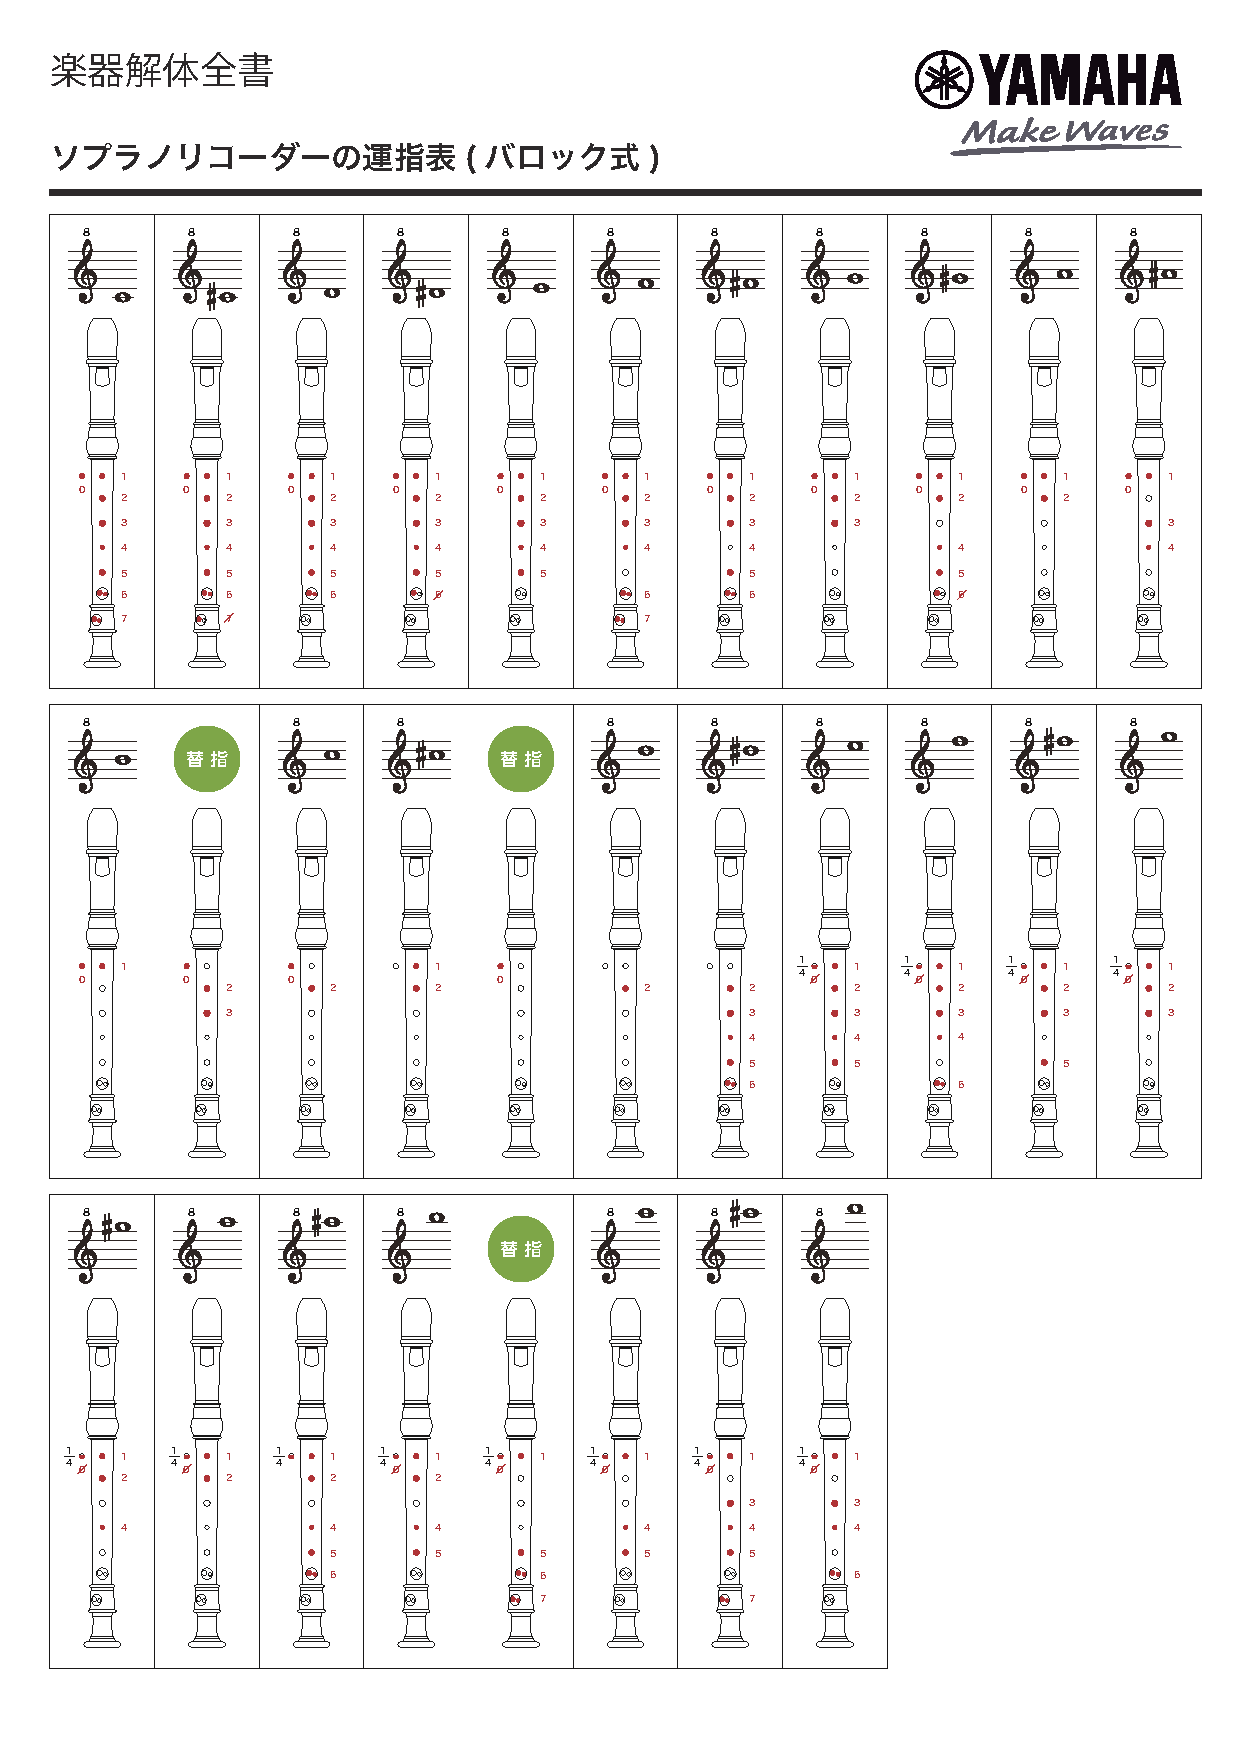
\includepdf[pages=-]{ソプラノリコーダー運指（ヤマハ）.pdf}
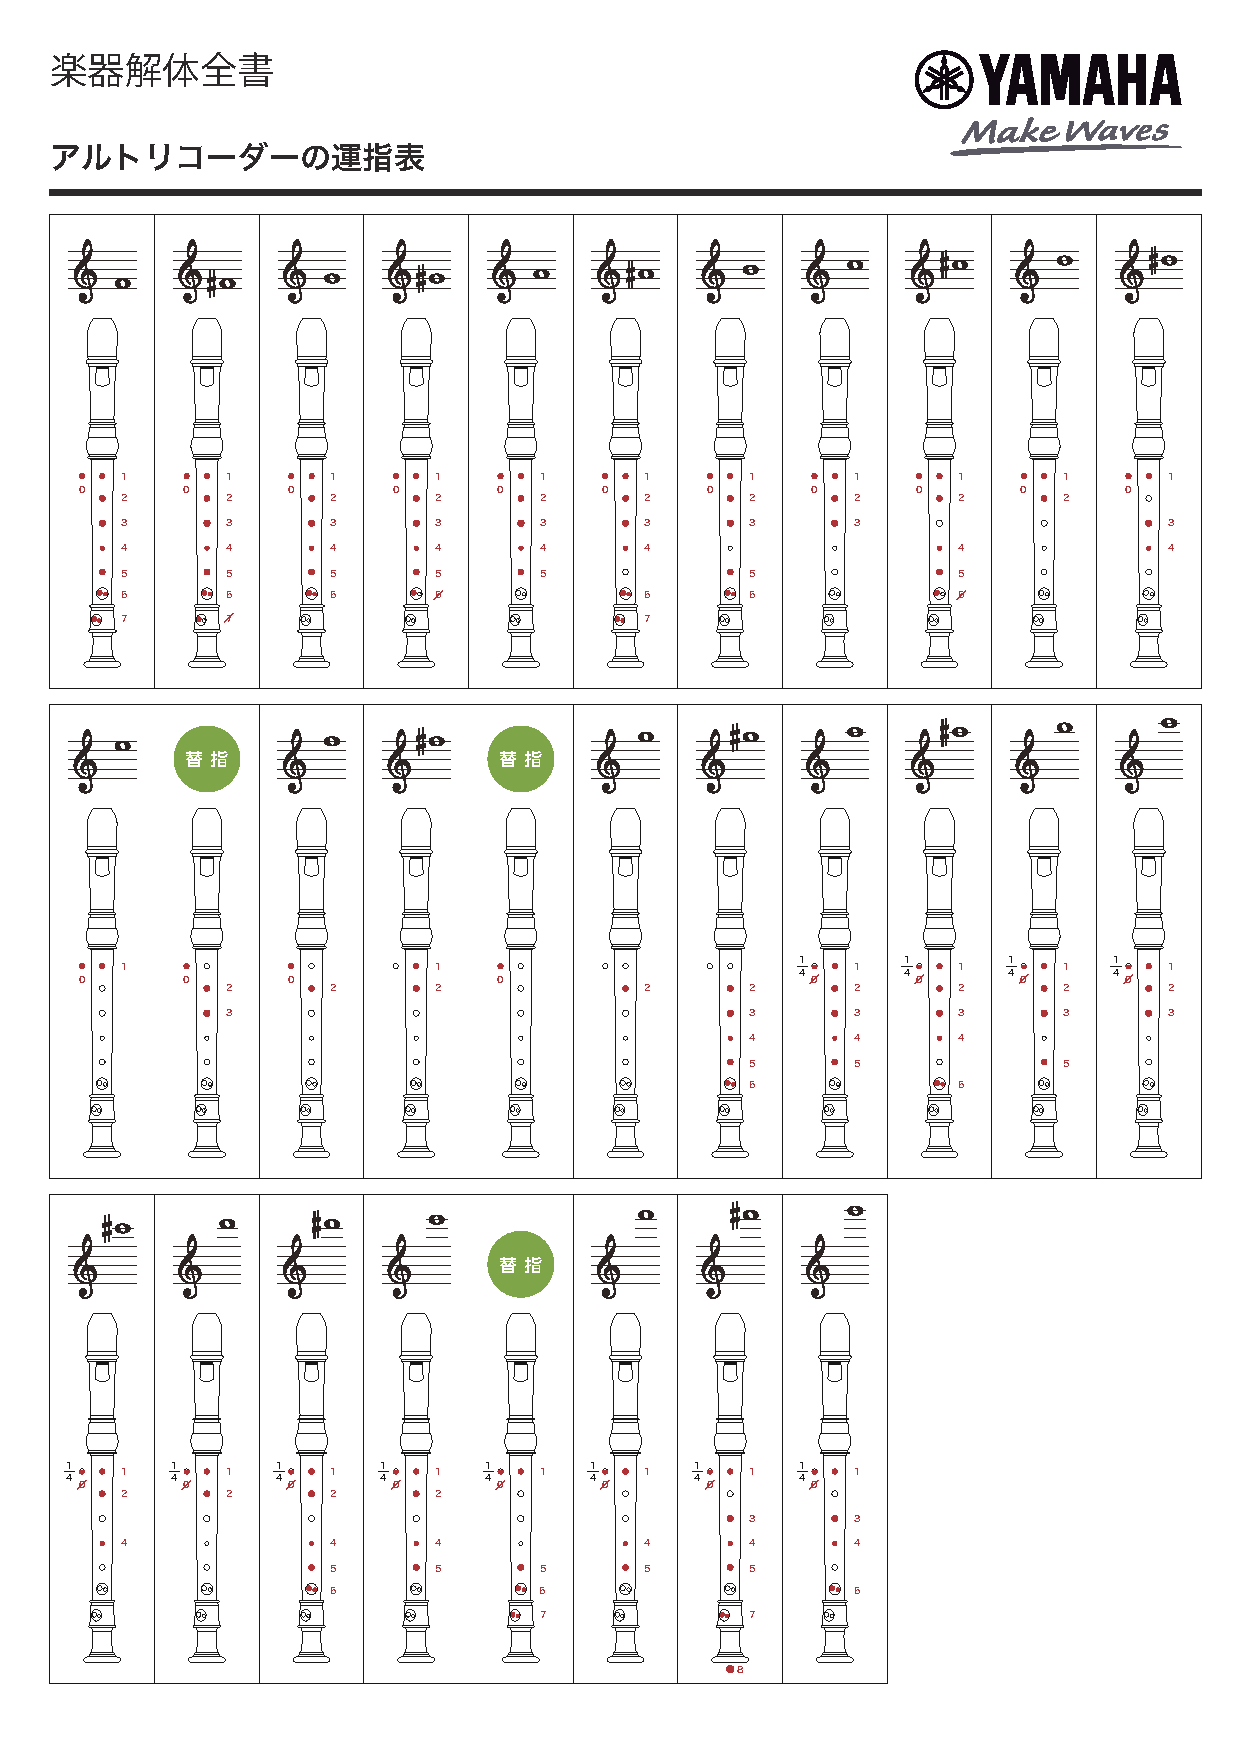
\includepdf[pages=-]{アルトリコーダー運指（ヤマハ）.pdf}

\end{document}
